\documentclass[border=6pt]{standalone}
\usepackage[T1]{fontenc}
\usepackage{courier}
\usepackage[scaled=0.95]{helvet}
\renewcommand{\familydefault}{\sfdefault}
\usepackage{sfmath}
\usepackage[version=4]{mhchem}
\usepackage{tikz}
\usepackage{pgfplots}
\pgfplotsset{compat=newest}
\usetikzlibrary{arrows.meta,positioning,calc,fit,backgrounds,shapes.geometric,decorations.pathreplacing,patterns}
\definecolor{ink}{HTML}{17233A}
\definecolor{inksoft}{HTML}{44506A}
\definecolor{teal}{HTML}{0E6B6B}
\definecolor{tealsoft}{HTML}{E5F0EF}
\definecolor{amber}{HTML}{B26B12}
\definecolor{ambersoft}{HTML}{FBF0DF}
\definecolor{blue}{HTML}{2F6690}
\definecolor{bluesoft}{HTML}{E3ECF4}
\definecolor{plum}{HTML}{7A4D8C}
\definecolor{plumsoft}{HTML}{EFE7F3}
\definecolor{greyc}{HTML}{8A94A3}
\definecolor{linec}{HTML}{D3DCE1}
\definecolor{oxy}{HTML}{C0392B}
\definecolor{carb}{HTML}{3B4252}
\definecolor{hyd}{HTML}{E6E9EE}
\definecolor{nit}{HTML}{2F6690}
\tikzset{
  every picture/.style={line cap=round,line join=round},
  lab/.style={font=\small, text=inksoft},
  >={Stealth[length=7pt]},
}
\pgfplotsset{
  every axis/.append style={axis line style={inksoft}, tick style={inksoft}, tick label style={font=\footnotesize, text=inksoft}, label style={font=\small, text=ink}},
}
% fragment tile: \frag{node name}{position}{colour}{content}
\newcommand{\frag}[4]{\node[draw=#3, fill=#3!12, line width=1.4pt, rounded corners=6pt, minimum width=1.25cm, minimum height=1.05cm, text=#3, font=\bfseries] (#1) at (#2) {#4};}
\newcommand{\ring}{\tikz[baseline=-0.6ex]{\draw[line width=1.1pt] (0:0.3)--(60:0.3)--(120:0.3)--(180:0.3)--(240:0.3)--(300:0.3)--cycle; \draw[line width=0.8pt] (0,0) circle (0.16);}}
\newcommand{\bond}[2]{\draw[ink, line width=2.2pt] (#1) -- (#2);}

\begin{document}
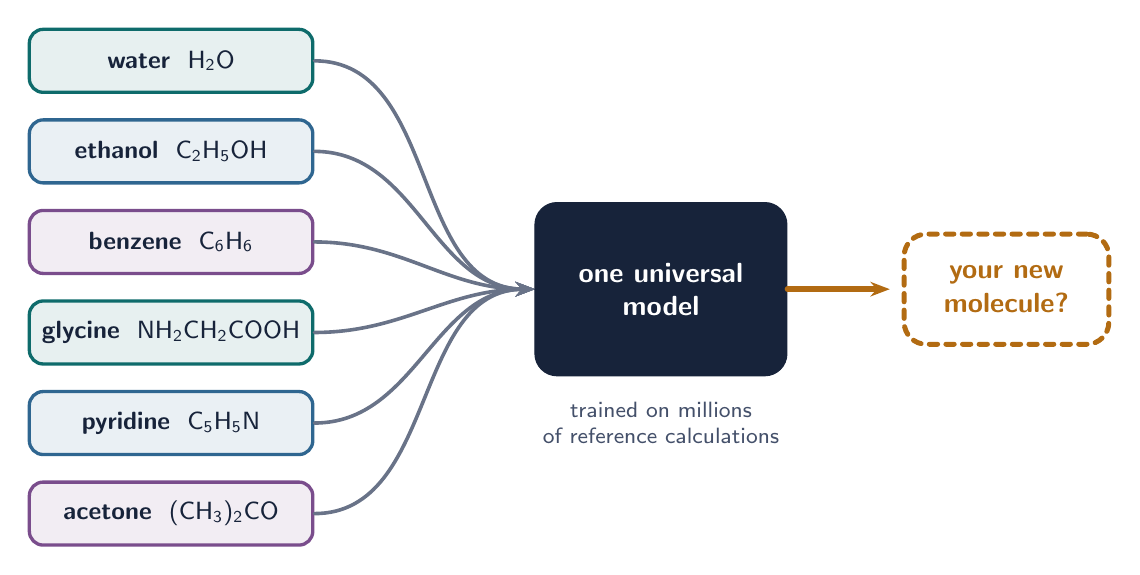
\begin{tikzpicture}
\node[draw=teal, fill=teal!10, line width=1.2pt, rounded corners=5pt, minimum width=3.6cm, minimum height=0.8cm, font=\small, text=ink, anchor=east] (m0) at (3.4,4.00) {\textbf{water}\ \ \ce{H2O}};
\draw[->, inksoft!80, line width=1.3pt] (m0.east) to[out=0, in=180] (6.2,1.1);
\node[draw=blue, fill=blue!10, line width=1.2pt, rounded corners=5pt, minimum width=3.6cm, minimum height=0.8cm, font=\small, text=ink, anchor=east] (m1) at (3.4,2.85) {\textbf{ethanol}\ \ \ce{C2H5OH}};
\draw[->, inksoft!80, line width=1.3pt] (m1.east) to[out=0, in=180] (6.2,1.1);
\node[draw=plum, fill=plum!10, line width=1.2pt, rounded corners=5pt, minimum width=3.6cm, minimum height=0.8cm, font=\small, text=ink, anchor=east] (m2) at (3.4,1.70) {\textbf{benzene}\ \ \ce{C6H6}};
\draw[->, inksoft!80, line width=1.3pt] (m2.east) to[out=0, in=180] (6.2,1.1);
\node[draw=teal, fill=teal!10, line width=1.2pt, rounded corners=5pt, minimum width=3.6cm, minimum height=0.8cm, font=\small, text=ink, anchor=east] (m3) at (3.4,0.55) {\textbf{glycine}\ \ \ce{NH2CH2COOH}};
\draw[->, inksoft!80, line width=1.3pt] (m3.east) to[out=0, in=180] (6.2,1.1);
\node[draw=blue, fill=blue!10, line width=1.2pt, rounded corners=5pt, minimum width=3.6cm, minimum height=0.8cm, font=\small, text=ink, anchor=east] (m4) at (3.4,-0.60) {\textbf{pyridine}\ \ \ce{C5H5N}};
\draw[->, inksoft!80, line width=1.3pt] (m4.east) to[out=0, in=180] (6.2,1.1);
\node[draw=plum, fill=plum!10, line width=1.2pt, rounded corners=5pt, minimum width=3.6cm, minimum height=0.8cm, font=\small, text=ink, anchor=east] (m5) at (3.4,-1.75) {\textbf{acetone}\ \ \ce{(CH3)2CO}};
\draw[->, inksoft!80, line width=1.3pt] (m5.east) to[out=0, in=180] (6.2,1.1);
\node[draw=ink, fill=ink, text=white, rounded corners=8pt, minimum width=3.2cm, minimum height=2.2cm, font=\bfseries, align=center] (u) at (7.8,1.1) {one universal\\model};
\node[font=\footnotesize, text=inksoft, align=center] at (7.8,-0.6) {trained on millions\\of reference calculations};
\draw[->, amber, line width=2pt] (u.east) -- ++(1.3,0);
\node[draw=amber, line width=1.8pt, dashed, rounded corners=8pt, minimum width=2.6cm, minimum height=1.4cm, font=\bfseries, text=amber, align=center, anchor=west] at ($(u.east)+(1.45,0)$) {your new\\molecule?};
\end{tikzpicture}
\end{document}
